\documentclass{report}

\input{../template/preamble}
\input{../template/macros}
\input{../template/letterfonts}

\usepackage{karnaugh-map}
\usepackage{tikz-timing}

\title{\Huge{Logic Circuits}\\Semester 5}
\author{\huge{Ahmad Abu Zainab}}
\date{}

\ctikzset{
	logic ports=ieee,
	logic ports/scale=0.7,
	logic ports/fill=lightgray,
    muxdemuxes/fill=lightgray,
    flipflops/fill=lightgray,
}

\begin{document}

\maketitle
\newpage% or \cleardoublepage
% \pdfbookmark[<level>]{<title>}{<dest>}
\pdfbookmark[section]{\contentsname}{toc}
\tableofcontents
\pagebreak

\chapter{Number Systems and Conversion}

\begin{itemize}
	\ii \textbf{Decimal} (Base 10): 0, 1, 2, 3, 4, 5, 6, 7, 8, 9
	\ii \textbf{Binary} (Base 2): 0, 1
	\ii \textbf{Octal} (Base 8): 0, 1, 2, 3, 4, 5, 6, 7
	\ii \textbf{Hexadecimal} (Base 16): 0, 1, 2, 3, 4, 5, 6, 7, 8, 9, A, B, C, D, E, F
\end{itemize}

\section{Decimal and Binary}

\subsection{Decimal to Binary}

\begin{enumerate}
	\ii Divide the decimal number by 2.
	\ii Keep the remainder.
	\ii Divide the quotient by 2.
	\ii Keep the remainder.
	\ii Repeat until the quotient is 0.
	\ii The binary number is the remainders in reverse order.
\end{enumerate}

If the number has a decimal point then we multiply the decimal part by 2 the integer part of the result is the binary digit and the decimal part is multiplied by 2 again and so on until we obtain only a 1.

\ex{
	Convert $53_{10}$ to binary.
}{
	\begin{align*}
		53/2 & = 26 \text{ remainder } 1 \\
		26/2 & = 13 \text{ remainder } 0 \\
		13/2 & = 6 \text{ remainder } 1  \\
		6/2  & = 3 \text{ remainder } 0  \\
		3/2  & = 1 \text{ remainder } 1  \\
		1/2  & = 0 \text{ remainder } 1  \\
	\end{align*}
	\[
		53_{10}  = 110101_2
		.\]
}

\ex{
	Convert $.625_{10}$ to binary
}{
	\begin{align*}
		.625 \times 2 & = 1.25 \\
		.25 \times 2  & = .5   \\
		.5 \times 2   & = 1    \\
	\end{align*}
	\[
		.625_{10} = .101_2
		.\]
}

\subsection{Binary to Decimal}

\begin{enumerate}
	\ii Write the binary number.
	\ii Multiply each digit by $2^n$ where $n$ is the position of the digit.
	\ii Add the results.
\end{enumerate}


\ex{
	Convert $110101_2$ to decimal.
}{
	\begin{align*}
		110101_2 & = 1 \times 2^5 + 1 \times 2^4 + 0 \times 2^3 + 1 \times 2^2 + 0 \times 2^1 + 1 \times 2^0 \\
		         & = 32 + 16 + 0 + 4 + 0 + 1                                                                 \\
		         & = 53_{10}
	\end{align*}
}

\section{Binary and Hexadecimal}

To convert from binary to hexadecimal we group the binary digits into groups of 4 starting from the right and convert each group to a hexadecimal digit.

\[
	1001101.010111_2 = \underbrace{0100}_{4} \underbrace{1101}_{D} . \underbrace{0101}_{5} \underbrace{1100}_{C} = 4D.5C_{16}
	.\]

\section{Operations on Binary Numbers}

\subsection{Addition}

\[
	\arraycolsep=1.4pt
	\begin{tabular}{r c c c}
		\text{carry} & 1 &   &   \\
		             & 0 & 1 & 1 \\
		+            & 1 & 1 & 0 \\
		\hline
		             & 1 & 0 & 1 \\
	\end{tabular}
	.\]

\subsection{Subtraction}

\[
	\arraycolsep=1.4pt
	\begin{tabular}{r c c c c c c c}
		\text{borrow} &   & 1 & 1 & 1 &   &   \\
		              & 1 & 1 & 1 & 0 & 0 & 1 \\
		-             &   &   & 1 & 0 & 1 & 1 \\
		\hline
		              & 1 & 0 & 1 & 1 & 1 & 0
	\end{tabular}
	.\]

\subsection{Multiplication}

\begin{align*}
	0\times 0 & = 0 \\
	0\times 0 & = 0 \\
	0\times 1 & = 0 \\
	1\times 1 & = 1 \\
\end{align*}

\[
	\arraycolsep=1.4pt
	\begin{tabular}{r c c c c c c c c c c}
		         &  &   &   &   &   & 1 & 1 & 0 & 1 \\
		$\times$ &  &   &   &   &   & 1 & 0 & 1 & 1 \\
		\hline
		         &  &   &   &   &   & 1 & 1 & 0 & 1 \\
		         &  &   &   &   & 1 & 1 & 0 & 1 &   \\
		         &  &   &   & 0 & 0 & 0 & 0 &   &   \\
		         &  &   & 1 & 1 & 0 & 1 &   &   &   \\
		\hline
		         &  & 1 & 0 & 0 & 0 & 1 & 1 & 1 & 1 \\
	\end{tabular}
	.\]

\subsection{Division}

Binary division is similar to decimal division, except it is much easier because the only two possible quotient digits are 0 and 1.

We start division by comparing the divisor with the upper bits of the dividend.

If we cannot subtract without getting a negative result, we move one place to the right and try again.

If we can subtract, we place a 1 for the quotient above the number we subtracted from and append the next dividend bit to the end of the difference and repeat this process with this modified difference until we run out of bits in the dividend.

\section{Negative Numbers in Binary}

\begin{description}
	\ii[Sign and Magnitude] The leftmost bit is the sign bit and the rest of the bits are the magnitude.
	\[
		-5_{10} = 1101_{2}
		.\]
	\ii[One's Complement] To negate a number we flip all the bits. $\bar{N} = (2^n-1) - N$ where $n$ is the number of bits.
	\[
		-5_{10} = (2^4 - 1) - 5 = 10_{10} = 1010_2
		.\]
	\ii[Two's Complement] To negate a number we flip all the bits and add 1. $N^* = 2^n - N$ where $n$ is the number of bits.
	\[
		-5_{10} = 2^4 - 5 = 11_{10} = 1011_2
		.\]
\end{description}

Adding a negative number in two's complement is the same as subtracting the positive number. In one's complement we add the numbers and add the carry to the result.

\chapter{Boolean Algebra}

\section{Logic Gates}

\begin{description}
	\ii[NOT Gate] The output is the inverse of the input.
	\[
		\begin{array}{c c}
			X & \bar{X} \\
			\hline
			0 & 1       \\
			1 & 0       \\
		\end{array}
		.\]
	\begin{figure}[H]
		\centering
		\begin{circuitikz}
			\draw (0,0) node[not port] (not) {};
			\draw (not.in) -- ++(-1,0) node[left] {$X$};
			\draw (not.out) -- ++(1,0) node[right] {$\bar{X}$};
		\end{circuitikz}
	\end{figure}
	\ii[AND Gate] The output is 1 if both inputs are 1.
	\[
		\begin{array}{c c c}
			X & Y & X \cdot Y \\
			\hline
			0 & 0 & 0         \\
			0 & 1 & 0         \\
			1 & 0 & 0         \\
			1 & 1 & 1         \\
		\end{array}
		.\]
	\begin{figure}[H]
		\centering
		\begin{circuitikz}
			\draw (0,0) node[and port] (and) {};
			\draw (and.in 1) -- ++(-1,0) node[left] {$X$};
			\draw (and.in 2) -- ++(-1,0) node[left] {$Y$};
			\draw (and.out) -- ++(1,0) node[right] {$X \cdot Y$};
		\end{circuitikz}
	\end{figure}

	\ii[OR Gate] The output is 1 if either input is 1.
	\[
		\begin{array}{c c c}
			X & Y & X + Y \\
			\hline
			0 & 0 & 0     \\
			0 & 1 & 1     \\
			1 & 0 & 1     \\
			1 & 1 & 1     \\
		\end{array}
		.\]
	\begin{figure}[H]
		\centering
		\begin{circuitikz}
			\draw (0,0) node[or port] (or) {};
			\draw (or.in 1) -- ++(-1,0) node[left] {$X$};
			\draw (or.in 2) -- ++(-1,0) node[left] {$Y$};
			\draw (or.out) -- ++(1,0) node[right] {$X + Y$};
		\end{circuitikz}
	\end{figure}

	\ii[XOR Gate] The output is 1 if either input is 1 but not both.
	\[
		\begin{array}{c c c}
			X & Y & X \oplus Y \\
			\hline
			0 & 0 & 0          \\
			0 & 1 & 1          \\
			1 & 0 & 1          \\
			1 & 1 & 0          \\
		\end{array}
		.\]
	\begin{figure}[H]
		\centering
		\begin{circuitikz}
			\draw (0,0) node[xor port] (xor) {};
			\draw (xor.in 1) -- ++(-1,0) node[left] {$X$};
			\draw (xor.in 2) -- ++(-1,0) node[left] {$Y$};
			\draw (xor.out) -- ++(1,0) node[right] {$X \oplus Y$};
		\end{circuitikz}
	\end{figure}

	\ii[Equivalence Gate] The output is 1 if both inputs are the same.
	\[
		\begin{array}{c c c}
			X & Y & X \equiv Y \\
			\hline
			0 & 0 & 1          \\
			0 & 1 & 0          \\
			1 & 0 & 0          \\
			1 & 1 & 1          \\
		\end{array}
		.\]
	\begin{figure}[H]
		\centering
		\begin{circuitikz}
			\draw (0,0) node[xnor port] (xnor) {};
			\draw (xnor.in 1) -- ++(-1,0) node[left] {$X$};
			\draw (xnor.in 2) -- ++(-1,0) node[left] {$Y$};
			\draw (xnor.out) -- ++(1,0) node[right] {$X \equiv Y$};
		\end{circuitikz}
	\end{figure}

\end{description}

\subsection{Switches}
If switch $X$ is open, then we will define the value of $X$ to be 0; if switch $X$ is closed, then we will define the value of $X$ to be 1.

\begin{figure}[H]
	\centering
	\begin{circuitikz}
		\draw (0,0) to[nos,l=$X$] (2,0);
	\end{circuitikz}
\end{figure}

\section{Laws and Theorems}

\begin{minipage}[t]{0.5\linewidth}
	\begin{itemize}

		\ii Operations involving 0 and 1
		\begin{align*}
			X + 0     & = X \\
			X + 1     & = 1 \\
			X \cdot 1 & = X \\
			X \cdot 0 & = 0 \\
		\end{align*}

		\ii Indempotent Laws
		\begin{align*}
			X + X     & = X \\
			X \cdot X & = X \\
		\end{align*}

		\ii Involution Law
		\[
			\overline{\bar{X}} = X
			.\]

		\ii Laws of complementation
		\begin{align*}
			X + \bar{X}     & = 1 \\
			X \cdot \bar{X} & = 0 \\
		\end{align*}

	\end{itemize}
\end{minipage}
\begin{minipage}[t]{0.4\linewidth}
	\begin{itemize}
		\ii Commutative Laws
		\begin{align*}
			X + Y     & = Y + X     \\
			X \cdot Y & = Y \cdot X \\
		\end{align*}

		\ii Associative Laws
		\begin{align*}
			X + (Y + Z)         & = (X + Y) + Z         \\
			X \cdot (Y \cdot Z) & = (X \cdot Y) \cdot Z \\
		\end{align*}

		\ii Distributive Laws
		\begin{align*}
			X \cdot (Y + Z)       & = X \cdot Y + X \cdot Z     \\
			X + Y \cdot Z         & = (X + Y) \cdot (X + Z)     \\
			X \cdot (Y+Z)         & = X\cdot Y + X \cdot Z      \\
			(X+Y)\cdot(X+Z)       & = X + Y \cdot Z             \\
			(X+Y)\cdot(\bar{X}+Z) & = X\cdot Z + \bar{X}\cdot Y
		\end{align*}

		\ii Simplification Laws
		\begin{align*}
			X \cdot Y + X \cdot \bar{Y} & = X         \\
			X + X\cdot Y                & = X         \\
			(X + \bar{Y}) \cdot Y       & = X \cdot Y \\
			(X + Y)\cdot(X + \bar{Y})   & = X         \\
			X \cdot (X + Y)             & = X         \\
			X \cdot \bar{Y} + Y         & = X + Y
		\end{align*}
	\end{itemize}
\end{minipage}

\begin{align*}
	X\oplus 0            & = X                                                                               \\
	X\oplus 1            & = \bar{X}                                                                         \\
	X\oplus X            & = 0                                                                               \\
	X\oplus \bar{X}      & = 1                                                                               \\
	X\oplus Y            & = Y\oplus X                                                                       \\
	X\oplus (Y\oplus Z)  & = (X\oplus Y)\oplus Z = X\oplus Y\oplus Z                                         \\
	X\cdot (Y\oplus Z)   & = X\cdot Y\oplus X\cdot Z                                                         \\
	\overline{X\oplus Y} & = \bar{X}\oplus Y = X\oplus \bar{Y} = X\cdot Y + \bar{X}\cdot \bar{Y} = X\equiv Y
\end{align*}

Consensus Theorem

\[
	X\cdot Y + \bar{X}\cdot Z + Y\cdot Z = X\cdot Y + \bar{X}\cdot Z
	.\]

in dual form

\[
	(X + Y)(\bar{X} + Z)(Y + Z) = (X + Y)(\bar{X} + Z)
	.\]


An expression is in sum of products form if it is a sum of products of literals.

\[
	A\bar{B} + C\bar{D}E + A\bar{C}\bar{E}
	.\]

Likewise, an expression is in product of sums form if it is a product of sums of literals.

\[
	(A + B)(C + D)E
	.\]

\section{De Morgan's Theorems}

\begin{align*}
	\overline{X + Y}     & = \bar{X} \cdot \bar{Y} \\
	\overline{X \cdot Y} & = \bar{X} + \bar{Y}
\end{align*}

\section{Duality}

Given an expression, we can obtain its dual by replacing all ANDs with ORs and all ORs with ANDs and all 0s with 1s and all 1s with 0s.

\begin{align*}
	(XYZ\cdots)^D         & = X + Y + Z + \cdots \\
	(X + Y + Z +\cdots)^D & = XYZ\cdots
\end{align*}

The dual can also be found by taking the complement of the whole expression then complementing each variable individually

\section{Minterm and Maxterm Expansions}

\begin{description}
	\ii[Minterm] A product term containing all the variables of the function in either true or complemented form.
	\ii[Maxterm] A sum term containing all the variables of the function in either true or complemented form.
\end{description}

Any Boolean function can be expressed as a sum of minterms or a product of maxterms.

\ex{Minterm}{
	\[
		f(A,B,C) =
		\underbrace{\bar{A}\bar{B}\bar{C}}_{000}+
		\underbrace{\bar{A}\bar{B}C}_{001}+
		\underbrace{\bar{A}BC}_{011}+
		\underbrace{\bar{A}B\bar{C}}_{010}+
		\underbrace{ABC}_{111}
		=
		\Sigma m(0,1,3,2,7)
		.\]
}

\ex{Maxterm}{
	\[
		f(A,B,C) =
		(\underbrace{\bar{A}+\bar{B}+\bar{C}}_{111})\cdot
		(\underbrace{\bar{A}+\bar{B}+C}_{110})\cdot
		(\underbrace{\bar{A}+B+C}_{100})\cdot
		(\underbrace{\bar{A}+B+\bar{C}}_{101})\cdot
		(\underbrace{A+B+C}_{000})
		=
		\Pi M(7,6,4,5,0)
		.\]
}

\chapter{Karnaugh Maps}

A Karnaugh map is a graphical representation of a truth table.\\

It is useful for simplifying Boolean expressions, by grouping together adjacent cells containing 1s.\\

We first draw a grid with the number of rows and columns equal to the number of variables.\\

We then label the rows and columns with the binary values of the variables using a Gray code. (000, 001, 011, 010, 110, 111, 101, 100) No 2 adjacent numbers differ by more than 1 bit\\

We then fill in the cells with the output of the function.\\

We then group together adjacent cells containing 1s in powers of 2 (1, 2, 4, 8, 16, 32, 64, 128, 256, etc.)\\

We then go over the groups and write down the variables that remain the same throughout the group.\\

\ex{Two Variable K-map}{
	Take the following K-map

	\begin{figure}[H]
	\centering
	\begin{karnaugh-map}(label=corner)[2][2][1][$A$][$B$]
	\minterms{0,2,3}
	\implicant{0}{2}
	\implicant{2}{3}
	\end{karnaugh-map}
	\end{figure}

	We look at the first group is 0 and 2(vertical), in this group $A$ is not changing and it's value is 0. So the first group corresponds to $\bar{A}$.\\

	The second group is 2 and 3(horizontal), in this group $B$ is not changing and it's value is 1. So the second group corresponds to $B$.\\

	Therefore the simplified expression is
	\[
		f(A,B) = \bar{A} + B
		.\]
}

\ex{Three Variable K-map}{
	Take the following function in min-term form
	\[
		f(A,B,C) = \Sigma m(0,1,3,4,6,7)
		.\]

	We can represent this function in a K-map as follows
	\begin{figure}[H]
	\centering
	\begin{karnaugh-map}(label=corner)[2][4][1][$A$][$C$][$B$]
	\minterms{0,1,2,5,6,7}
	\implicant{0}{1}
	\implicant{7}{5}
	\implicant{2}{6}
	\end{karnaugh-map}
	\end{figure}

	First group(red) the only changing variable is $A$. So it's excluded in the term of the group which is $\bar{B}\bar{C}$.\\
	Second group(yellow) the only changing variable is $B$. So it's excluded in the term of the group which is $\bar{A}C$.\\
	Third group(green) the only changing variable is $C$. So it's excluded in the term of the group which is $AB$.\\

	Therefore the simplified expression is
	\[
		f(A,B,C) = \bar{B}\bar{C} + \bar{A}C + AB
		.\]
}

\ex{Four Variable K-map}{
	Take the following function in min-term form
	\[
		f(A,B,C,D) = \Sigma m(0,2,4,5,8,10,12,13)
		.\]

	We can represent this function in a K-map as follows
	\begin{figure}[H]
	\centering
	\begin{karnaugh-map}[4][4][1][$AB$][$CD$]
	\minterms{0,1,2,3,5,7,8,10}
	\implicant{1}{7}
	\implicant{1}{7}
	\implicantcorner
	\end{karnaugh-map}
	\begin{karnaugh-map}[4][4][1][$AB$][$CD$]
	\minterms{0,1,2,3,5,7,8,10}
	\implicant{0}{2}
	\implicant{5}{7}
	\implicantedge{8}{8}{10}{10}
	\end{karnaugh-map}
	\end{figure}

	First K-map gives us the simplified form as
	\[
		f(A,B,C,D) = B\bar{C} + \bar{B}\bar{D}
		.\]

	And the second K-map gives us
	\[
		f(A,B,C,D) = \bar{C}\bar{D} + B\bar{C}D + \bar{B}C\bar{D}
		.\]
}

To untilize maxterms in a K-map we first fill the maxterm cells with 0s and the rest with 1s, and then we follow the same procedure as before. This will give us $\bar{f}$ then we simply compute the inverse to get $f$.

\nt{
	Sometimes we don't care about some of the outputs of a function (Don't care conditions). We can represent this in a K-map by filling the cells with don't care conditions with an X. An example is
	\[
		f(A,B,C) = \Sigma m(0,1,3,4,5,7) + d(2,6)
		.\]
}

\chapter{Combinational Logic}

\begin{description}
	\ii[Combinational Logic] A logic circuit whose output depends only on the current input values.
	\ii[Sequential Logic] A logic circuit whose output depends on the current input values and the past input values.
\end{description}

The maximum number of gates cascaded in series between a circuit input and the output is referred to as the number of \emph{levels} of gates.

\ex{}{
	We need to realize the 2 level circuit and the 3 level circuit. The 2 level circuit is realized by cascading 2 gates in series and the 3 level circuit is realized by cascading 3 gates in series.
	\[
		f(a,b,c,d) = \Sigma m(1, 5, 6, 10, 13, 14)
		.\]

	First we construct the k-map

	\begin{figure}[H]
	\centering
	\begin{karnaugh-map}(label=corner)[4][4][1][$AB$][$CD$]
	\minterms{4,5,7,9,10,11}
	\implicant{4}{5}
	\implicant{5}{7}
	\implicant{9}{11}
	\implicant{11}{10}
	\end{karnaugh-map}
	\end{figure}

	Giving us
	\[
		f = a'c'd + bc'd + bcd' + acd'
		.\]

	Yielding the following circuit

	\begin{figure}[H]
		\centering
		\begin{circuitikz}
			% \draw (0,0) node[xor port , number inputs=3](XOR1){};
			\draw (0,0) node[and port , number inputs=3](AND1){};
			\draw (AND1.in 1) -- ++(0,0) node[left]{$a'$};
			\draw (AND1.in 2) -- ++(0,0) node[left]{$c'$};
			\draw (AND1.in 3) -- ++(0,0) node[left]{$d$};

			\draw (0,-1) node[and port , number inputs=3](AND2){};
			\draw (AND2.in 1) -- ++(0,0) node[left]{$b$};
			\draw (AND2.in 2) -- ++(0,0) node[left]{$c'$};
			\draw (AND2.in 3) -- ++(0,0) node[left]{$d$};

			\draw (0,-2) node[and port , number inputs=3](AND3){};
			\draw (AND3.in 1) -- ++(0,0) node[left]{$b$};
			\draw (AND3.in 2) -- ++(0,0) node[left]{$c$};
			\draw (AND3.in 3) -- ++(0,0) node[left]{$d'$};

			\draw (0,-3) node[and port , number inputs=3](AND4){};
			\draw (AND4.in 1) -- ++(0,0) node[left]{$a$};
			\draw (AND4.in 2) -- ++(0,0) node[left]{$c$};
			\draw (AND4.in 3) -- ++(0,0) node[left]{$d'$};

			\draw (3, -1.5) node[or port , number inputs=4](OR1){};
			\draw (AND1.out) -- ++(1,0) |- (OR1.in 1);
			\draw (AND2.out) -- ++(0.5,0) |- (OR1.in 2);
			\draw (AND3.out) -- ++(0.5,0) |- (OR1.in 3);
			\draw (AND4.out) -- ++(1,0) |- (OR1.in 4);
			\draw (OR1.out) -- ++(1,0) node[right]{$f$};
		\end{circuitikz}
	\end{figure}

	The 3 level circuit is realized by cascading 3 gates in series. We obtain the expression for the 3 level circuit by factoring $f$ as follows

	\[
		f = c'd(a' + b) + cd'(a + b)
		.\]

	Giving us the following circuit
	\begin{figure}[H]
		\centering
		\begin{circuitikz}
			\draw (0,0) node[or port , number inputs=2](OR1){};
			\draw (OR1.in 1) -- ++(0,0) node[left]{$a'$};
			\draw (OR1.in 2) -- ++(0,0) node[left]{$b$};

			\draw (2,-1) node[and port , number inputs=3](AND1){};
			\draw (OR1.out) |- (AND1.in 1);
			\draw (AND1.in 2) -- ++(0,0) node[left]{$c'$};
			\draw (AND1.in 3) -- ++(0,0) node[left]{$d$};

			\draw (0,-2) node[or port , number inputs=2](OR2){};
			\draw (OR2.in 1) -- ++(0,0) node[left]{$a$};
			\draw (OR2.in 2) -- ++(0,0) node[left]{$b$};

			\draw (2,-3) node[and port , number inputs=3](AND2){};
			\draw (OR2.out) |- (AND2.in 1);
			\draw (AND2.in 2) -- ++(0,0) node[left]{$c$};
			\draw (AND2.in 3) -- ++(0,0) node[left]{$d'$};

			\draw (3.5,-2) node[or port , number inputs=2](OR3){};
			\draw (AND1.out) |- (OR3.in 1);
			\draw (AND2.out) |- (OR3.in 2);
			\draw (OR3.out) -- ++(1,0) node[right]{$f$};
		\end{circuitikz}
	\end{figure}

	We do this again for max-term form. Then we compare all the circuits and choose the one with the least number of gates.
}

\section{NAND and NOR Gates}

\begin{description}
	\ii[NAND Gate] The output is 0 if both inputs are 1.
	\[
		\begin{array}{c c c}
			X & Y & X \uparrow Y \\
			\hline
			0 & 0 & 1            \\
			0 & 1 & 1            \\
			1 & 0 & 1            \\
			1 & 1 & 0            \\
		\end{array}
		.\]
	\begin{figure}[H]
		\centering
		\begin{circuitikz}
			\draw (0,0) node[nand port] (nand) {};
			\draw (nand.in 1) -- ++(-1,0) node[left] {$X$};
			\draw (nand.in 2) -- ++(-1,0) node[left] {$Y$};
			\draw (nand.out) -- ++(1,0) node[right] {$X \uparrow Y$};
		\end{circuitikz}
	\end{figure}

	\ii[NOR Gate] The output is 1 if both inputs are 0.
	\[
		\begin{array}{c c c}
			X & Y & X \downarrow Y \\
			\hline
			0 & 0 & 1              \\
			0 & 1 & 0              \\
			1 & 0 & 0              \\
			1 & 1 & 0              \\
		\end{array}
		.\]
	\begin{figure}[H]
		\centering
		\begin{circuitikz}
			\draw (0,0) node[nor port] (nor) {};
			\draw (nor.in 1) -- ++(-1,0) node[left] {$X$};
			\draw (nor.in 2) -- ++(-1,0) node[left] {$Y$};
			\draw (nor.out) -- ++(1,0) node[right] {$X \downarrow Y$};
		\end{circuitikz}
	\end{figure}
\end{description}

A set of gates is said to be functionally complete if all Boolean functions can be realized using only gates from the set.
AND and NOT gates are functionally complete since we can realize all Boolean functions using only AND and NOT gates (including OR).\\

Since we can realize AND and NOT gates using only NAND gates, NAND gates are also functionally complete.\\

\begin{enumerate}
	\ii \textbf{NOT}
	\begin{figure}[H]
		\centering
		\begin{circuitikz}
			\draw (0,0) node[nand port] (nand) {};
			\draw (nand.in 1) -- ++(-0.5,0) node[left] {$X$};
			\draw (nand.in 2) |- (nand.in 1);
			\draw (nand.out) -- ++(0.5,0) node[right] {$\bar{X}$};
		\end{circuitikz}
	\end{figure}

	\ii \textbf{AND}
	\begin{figure}[H]
		\centering
		\begin{circuitikz}
			\draw (0,0) node[nand port] (nand1) {};
			\draw (nand1.in 1) -- ++(-0.5,0) node[left] {$X$};
			\draw (nand1.in 2) -- ++(-0.5,0) node[left] {$Y$};
			\draw (2,0) node[nand port] (nand2) {};
			\draw (nand2.in 1) |- (nand1.out);
			\draw (nand2.in 2) |- (nand2.in 1);
			\draw (nand2.out) -- ++(0.5,0) node[right] {$X \cdot Y$};
		\end{circuitikz}
	\end{figure}

	\ii \textbf{OR}
	\begin{figure}[H]
		\centering
		\begin{circuitikz}
			\draw (0,0) node[nand port] (nand1) {};
			\draw (nand1.in 1) -- ++(-0.5,0) node[left] {$X$};
			\draw (nand1.in 2) |- (nand1.in 1);
			\draw (0,-1) node[nand port] (nand2) {};
			\draw (nand2.in 1) -- ++(-0.5,0) node[left] {$Y$};
			\draw (nand2.in 2) |- (nand2.in 1);
			\draw (2,-0.5) node[nand port] (nand3) {};
			\draw (nand3.in 1) |- (nand1.out);
			\draw (nand3.in 2) |- (nand2.out);
			\draw (nand3.out) -- ++(0.5,0) node[right] {$X + Y$};
		\end{circuitikz}
	\end{figure}
\end{enumerate}

\section{Design of Two-Level NAND and NOR-Gate Circuits}

A circuit composed of AND and OR gates can be converted to a circuit composed of NAND and NOR gates by using the formula $f = \overline{f'}$.\\

\ex{}{
	Given the function
	\[
		F = A + BC' + B'CD
		.\]

	We can convert it to several forms
	\begin{align*}
		F & = [(A + BC' + B'CD)']' \quad                      & \text{AND-OR}    \\
		  & = [A' \cdot (B + C')' \cdot (B' + C + D)']' \quad & \text{NAND-NAND} \\
		  & = [A' \cdot (B' + C) \cdot (B + C' + D')]' \quad  & \text{OR-NAND}   \\
		  & = A + (B' + C)' + (B + C' + D')' \quad            & \text{NOR-OR}
	\end{align*}
}

The procedure for designing a two-level NAND-NAND circuit is as follows

\begin{enumerate}
	\ii Find a minimum sum-of-products expression for F.
	\ii Draw the corresponding two-level AND-OR circuit.
	\ii Replace all gates with NAND gates leaving the gate interconnections unchanged.
	\ii If the output gate has any single literals as inputs, complement these literals.
\end{enumerate}

The procedure for designing a two-level NOR-NOR circuit is as follows

\begin{enumerate}
	\ii Find a minimum product-of-sums expression for F.
	\ii Draw the corresponding two-level OR-AND circuit.
	\ii Replace all gates with NOR gates leaving the gate interconnections unchanged.
	\ii If the output gate has any single literals as inputs, complement these literals.
\end{enumerate}

To design a multi-level NAND-gate circuit we perform the following procedure

\begin{enumerate}
	\ii Simplify the function.
	\ii Draw the corresponding AND-OR circuit. The output gate should be an OR gate.
	\ii Replace all gates with NAND gates leaving the gate interconnections unchanged.
	\ii Take the output-gate at level 1. The literal inputs to even levels remain unchanged while the literal inputs to odd levels are complemented.
\end{enumerate}

\subsection{Alternative Representations}
We will sometimes use a shorter circuit representation
% circuit using notcirc
\begin{figure}[H]
	\centering
	\begin{circuitikz}
		\draw (0,0) node[buffer port] (not) {};
		\draw (not.out) -- ++(1,0) node[right] {$X$};
		\draw (not.in) -- ++(-1,0) node[left] {$\bar{X}$};
		% \node at (not.in) [circleinv] {};
		\draw (not.bin) node[notcirc,left] {};
	\end{circuitikz}
\end{figure}
to represent a circuit using a NOT gate.
\begin{enumerate}
	\ii \textbf{AND}
	\begin{figure}[H]
		\centering
		\begin{circuitikz}
			\draw (0,0) node[nor port] (nor) {};
			\draw (nor.in 1) -- ++(-0.5,0) node[left] {$X$};
			\draw (nor.in 2) -- ++(-0.5,0) node[left] {$Y$};
			\draw (nor.out) -- ++(0.5,0) node[right] {$(X' + Y')' = X \cdot Y$};
			\draw (nor.bin 1) node[notcirc, left] {};
			\draw (nor.bin 2) node[notcirc, left] {};
		\end{circuitikz}
	\end{figure}

	\ii \textbf{OR}
	\begin{figure}[H]
		\centering
		\begin{circuitikz}
			\draw (0,0) node[nand port] (nand) {};
			\draw (nand.in 1) -- ++(-0.5,0) node[left] {$X$};
			\draw (nand.in 2) -- ++(-0.5,0) node[left] {$Y$};
			\draw (nand.out) -- ++(0.5,0) node[right] {$(X' \cdot Y')' = X + Y$};
			\draw (nand.bin 1) node[notcirc, left] {};
			\draw (nand.bin 2) node[notcirc, left] {};
		\end{circuitikz}
	\end{figure}

	\ii \textbf{NAND}
	\begin{figure}[H]
		\centering
		\begin{circuitikz}
			\draw (0,0) node[or port] (or) {};
			\draw (or.in 1) -- ++(-0.5,0) node[left] {$X$};
			\draw (or.in 2) -- ++(-0.5,0) node[left] {$Y$};
			\draw (or.out) -- ++(0.5,0) node[right] {$X' + Y' = X \uparrow Y$};
			\draw (or.bin 1) node[notcirc, left] {};
			\draw (or.bin 2) node[notcirc, left] {};
		\end{circuitikz}
	\end{figure}

	\ii \textbf{NOR}
	\begin{figure}[H]
		\centering
		\begin{circuitikz}
			\draw (0,0) node[and port] (and) {};
			\draw (and.in 1) -- ++(-0.5,0) node[left] {$X$};
			\draw (and.in 2) -- ++(-0.5,0) node[left] {$Y$};
			\draw (and.out) -- ++(0.5,0) node[right] {$X' \cdot Y' = X \downarrow Y$};
			\draw (and.bin 1) node[notcirc, left] {};
			\draw (and.bin 2) node[notcirc, left] {};
		\end{circuitikz}
	\end{figure}
\end{enumerate}

These alternative representations are useful for simplifying circuits when converting to and from NAND-NAND and AND-OR.

The following procedure may be used to convert to a NAND (or NOR) circuit:

\begin{enumerate}
	\ii We add an inversion bubble to the input of the odd levels.
	\ii If an inverted input is connected to an inverted output, we leave it as is.
	\ii If an inverted input is connected to a non-inverted output (or vice-versa), we add an inversion bubble to the non-inverted terminal to cancel the inversion.
	\ii If a literal is connected to an inverted input, we complement the literal.
\end{enumerate}

\section{Design of Combinational Circuits}

Digital design systems' solution often requires implementing multiple functions. While we can implement each function separately, it is often more efficient to implement all the functions together.\\

\ex{}{
	We need to implement the following functions
	\begin{align*}
		f_1 & = \Sigma m(11, 12, 13, 14, 15)   \\
		f_2 & = \Sigma m(3, 7, 11, 12, 13, 15) \\
		f_3 & = \Sigma m(3, 7, 12, 13, 14, 15)
	\end{align*}

	We can implement each function separately as follows
	\begin{figure}[H]
	\centering
	\resizebox{0.28\linewidth}{!}{
		\begin{karnaugh-map}(label=corner)[4][4][1][$AB$][$CD$]
		\minterms{11,14,15,3,7}
		\implicant{15}{14}
		\implicant{3}{11}
		\end{karnaugh-map}
	}

	\resizebox{0.28\linewidth}{!}{
		\begin{karnaugh-map}(label=corner)[4][4][1][$AB$][$CD$]
		\minterms{12,13,14,15,3,7}
		\implicant{12}{14}
		\implicant{3}{7}
		\end{karnaugh-map}
	}
	\resizebox{0.28\linewidth}{!}{
		\begin{karnaugh-map}(label=corner)[4][4][1][$AB$][$CD$]
		\minterms{12,13,15,3,7,11}
		\implicant{12}{13}
		\implicant{3}{11}
		\end{karnaugh-map}
	}
	\end{figure}

	\begin{align*}
		f_1 & = ab + acd  \\
		f_2 & = abc' + cd \\
		f_3 & = a'cd + ab
	\end{align*}

	The obtained circuit for all 3 separately looks like
	\begin{figure}[H]
		\centering
		\begin{circuitikz}
			\draw (0,0) node[and port, number inputs=3] (AND1) {};
			\draw (AND1.in 1) -- ++(-0.5,0) node[left] {$a$};
			\draw (AND1.in 2) -- ++(-0.5,0) node[left] {$c$};
			\draw (AND1.in 3) -- ++(-0.5,0) node[left] {$d$};

			\draw (0,-1) node[and port] (AND2) {};
			\draw (AND2.in 1) -- ++(-0.5,0) node[left] {$a$};
			\draw (AND2.in 2) -- ++(-0.5,0) node[left] {$b$};

			\draw (1.5,-0.5) node[or port] (OR1) {};
			\draw (AND1.out) |- (OR1.in 1);
			\draw (AND2.out) |- (OR1.in 2);
			\draw (OR1.out) -- ++(0.5,0) node[right] {$f_1$};

			\draw (0,-2) node[and port, number inputs=3] (AND3) {};
			\draw (AND3.in 1) -- ++(-0.5,0) node[left] {$a$};
			\draw (AND3.in 2) -- ++(-0.5,0) node[left] {$b$};
			\draw (AND3.in 3) -- ++(-0.5,0) node[left] {$c'$};

			\draw (0,-3) node[and port] (AND4) {};
			\draw (AND4.in 1) -- ++(-0.5,0) node[left] {$c$};
			\draw (AND4.in 2) -- ++(-0.5,0) node[left] {$d$};

			\draw (1.5,-2.5) node[or port] (OR2) {};
			\draw (AND3.out) |- (OR2.in 1);
			\draw (AND4.out) |- (OR2.in 2);
			\draw (OR2.out) -- ++(0.5,0) node[right] {$f_2$};

			\draw (0,-4) node[and port, number inputs=3] (AND5) {};
			\draw (AND5.in 1) -- ++(-0.5,0) node[left] {$a'$};
			\draw (AND5.in 2) -- ++(-0.5,0) node[left] {$c$};
			\draw (AND5.in 3) -- ++(-0.5,0) node[left] {$d$};

			\draw (0,-5) node[and port] (AND6) {};
			\draw (AND6.in 1) -- ++(-0.5,0) node[left] {$a$};
			\draw (AND6.in 2) -- ++(-0.5,0) node[left] {$b$};

			\draw (1.5,-4.5) node[or port] (OR3) {};
			\draw (AND5.out) |- (OR3.in 1);
			\draw (AND6.out) |- (OR3.in 2);
			\draw (OR3.out) -- ++(0.5,0) node[right] {$f_3$};
		\end{circuitikz}
	\end{figure}

	By grouping terms we can simplify the circuit to

	\begin{figure}[H]
		\centering
		\begin{circuitikz}
			\draw (0,0) node[and port] (AND1) {};
			\draw (AND1.in 1) -- ++(-0.5,0) node[left] {$a$};
			\draw (AND1.in 2) -- ++(-0.5,0) node[left] {$b$};

			\draw (0,-1) node[and port, number inputs=3] (AND2) {};
			\draw (AND2.in 1) -- ++(-0.5,0) node[left] {$a$};
			\draw (AND2.in 2) -- ++(-0.5,0) node[left] {$c$};
			\draw (AND2.in 3) -- ++(-0.5,0) node[left] {$d$};

			\draw (0,-2) node[and port, number inputs=3] (AND3) {};
			\draw (AND3.in 1) -- ++(-0.5,0) node[left] {$a$};
			\draw (AND3.in 2) -- ++(-0.5,0) node[left] {$b$};
			\draw (AND3.in 3) -- ++(-0.5,0) node[left] {$c'$};

			\draw (0,-3) node[and port, number inputs=3] (AND4) {};
			\draw (AND4.in 1) -- ++(-0.5,0) node[left] {$a'$};
			\draw (AND4.in 2) -- ++(-0.5,0) node[left] {$c$};
			\draw (AND4.in 3) -- ++(-0.5,0) node[left] {$d$};

			\draw (2,-0.5) node[or port] (OR1) {};
			\draw (AND1.out) |- (OR1.in 1);
			\draw (OR1.out) -- ++(0.5,0) node[right] {$f_1$};

			\draw (2,-1.5) node[or port, number inputs=3] (OR2) {};
			\draw (AND2.out) |- (OR2.in 1) node[pos=0.7] (JUNC1) {};
			\draw (AND3.out) |- (OR2.in 2);
			\draw (OR2.out) -- ++(0.5,0) node[right] {$f_2$};

			\draw (2,-2.5) node[or port] (OR3) {};
			\draw (AND4.out) |- (OR3.in 1);
			\draw (OR3.out) -- ++(0.5,0) node[right] {$f_3$};

			\draw (JUNC1) to[short,*-] ++(0,0) |- (OR1.in 2);
			\draw (OR1.in 1) ++(-0.1,0) to[short,*-] ++(0,0) |- (OR3.in 2);
			\draw (OR2.in 3) to[short, -*] (OR3.in 1);
		\end{circuitikz}
	\end{figure}

	The simplified circuit has 7 gates while the original circuit has 9 gates.
}

\section{Design of Circuits with Limited Gate Fan-In}

When designing a circuit we may be limited by the number of inputs a gate can have. We can overcome this by factoring the function into a multi-level circuit.\\

\ex{}{
	We need to implement the following function using only 3 input NOR gates.
	\[
		f = \Sigma m(0, 3, 4, 5, 8, 9, 10, 14, 15)
		.\]

	\begin{figure}[H]
	\centering
	\begin{karnaugh-map}(label=corner)[4][4][1][$AB$][$CD$]
	\maxterms{3,4,7,8,9,13,14}
	\minterms{0,1,2,5,6,12,15,10,11}
	\implicant{4}{4}
	\implicant{3}{7}
	\implicant{8}{9}
	\implicant{13}{9}
	\implicant{14}{14}
	\end{karnaugh-map}
	\end{figure}

	The simplest form (two-level) requires 2 4-input gate and 1 5-input gate. We can factor the function to remedy this

	\begin{align*}
		f' & = b'd(a'c' + ac) + a'c(b+d') + abc'                      \\
		f  & = [b + d' + (a + c)(a' + c')][a + c' + b'd][a' + b' + c]
	\end{align*}

	\begin{figure}[H]
		\centering
		\begin{circuitikz}
			\draw (0,0) node[nor port] (NOR1) {};
			\draw (NOR1.in 1) -- ++(-0.25,0) node[left] {$a$};
			\draw (NOR1.in 2) -- ++(-0.25,0) node[left] {$c$};

			\draw (0,-1) node[nor port] (NOR2) {};
			\draw (NOR2.in 1) -- ++(-0.25,0) node[left] {$a'$};
			\draw (NOR2.in 2) -- ++(-0.25,0) node[left] {$c'$};

			\draw (2,1) node[nor port] (NOR3) {};
			\draw (NOR3.in 1) -- ++(-0.25,0) node[left] {$b$};
			\draw (NOR3.in 2) -- ++(-0.25,0) node[left] {$d'$};

			\draw (2,-0.5) node[nor port] (NOR4) {};
			\draw (NOR1.out) |- (NOR4.in 1);
			\draw (NOR2.out) |- (NOR4.in 2);

			\draw (4,1.5) node[nor port, number inputs=3] (NOR5) {};
			\draw (NOR5.in 1) -- ++(-0.25,0) node[left] {$a$};
			\draw (NOR5.in 2) -- ++(-0.25,0) node[left] {$c'$};
			\draw (NOR3.out) |- (NOR5.in 3);

			\draw (4,0.5) node[nor port, number inputs=3] (NOR6) {};
			\draw (NOR6.in 1) -- ++(-0.25,0) node[left] {$a'$};
			\draw (NOR6.in 2) -- ++(-0.25,0) node[left] {$b'$};
			\draw (NOR6.in 3) -- ++(-0.25,0) node[left] {$c$};

			\draw (4,-0.5) node[nor port, number inputs=3] (NOR7) {};
			\draw (NOR7.in 1) -- ++(-0.25,0) node[left] {$b$};
			\draw (NOR4.out) |- (NOR7.in 2);
			\draw (NOR7.in 3) -- ++(-0.25,0) node[left] {$d'$};

			\draw (6,0.5) node[nor port, number inputs=3] (NOR8) {};
			\draw (NOR5.out) |- (NOR8.in 1);
			\draw (NOR6.out) |- (NOR8.in 2);
			\draw (NOR7.out) |- (NOR8.in 3);
			\draw (NOR8.out) -- ++(0.25,0) node[right] {$f$};
		\end{circuitikz}
	\end{figure}
}

\section{Gate Delays and Timing Diagrams}

\begin{figure}[H]
	\centering
	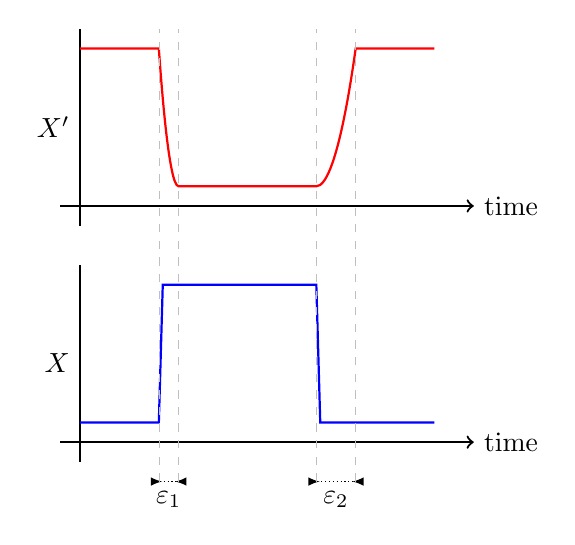
\begin{tikzpicture}
		% X
		\draw[->,thick] (-0.25,0)--(5,0) node[right]{time};
		\draw[thick] (0,-0.25)--(0,2.25) node[left, pos=0.5]{$X$};
		\draw[blue, thick] (0,0.25) -- (1,0.25) --  (1.05,2) -- (3,2) -- (3.05,0.25) -- (4.5,0.25);

		% X'
		\draw[->,thick] (-0.25,3)--(5,3) node[right]{time};
		\draw[thick] (0,-0.25+3)--(0,5.25) node[left, pos=0.5]{$X'$};
		\draw[red, thick] (0,5) -- (1,5) parabola[bend at end] (1.25,3.25) -- (3,3.25) parabola (3.5,5) -- (4.5,5);

		% Error label 
		\draw[{latex[reversed]}-{latex[reversed]}, densely dotted] (0.9,-0.5) -- (1.35,-0.5) node[below, pos=0.5] () {$\varepsilon_1$};
		\draw[help lines, color=gray!50, dashed] (1,-0.5) -- (1,5.25);
		\draw[help lines, color=gray!50, dashed] (1.25,-0.5) -- (1.25,5.25);

		\draw[{latex[reversed]}-{latex[reversed]}, densely dotted] (2.9,-0.5) -- (3.6,-0.5) node[below, pos=0.5] () {$\varepsilon_2$};
		\draw[help lines, color=gray!50, dashed] (3,-0.5) -- (3,5.25);
		\draw[help lines, color=gray!50, dashed] (3.5,-0.5) -- (3.5,5.25);
	\end{tikzpicture}
\end{figure}

\chapter{Multiplexers, Decoders, and Programmable Logic Devices}

\section{Multiplexers}

A multiplexer is a combinational circuit that selects one of many inputs and directs it to a single output.

\begin{figure}[H]
	\centering
	\begin{circuitikz}
		\draw (0,0) node[muxdemux , muxdemux def={NL=2, NR=1, NB=1, w=1.5, Lh=2, Rh=1, square pins=1}] (MUX) {};
		\draw (MUX.lpin 1) -- ++(-0.5,0) node[left] {$I_0$};
		\draw (MUX.lpin 2) -- ++(-0.5,0) node[left] {$I_1$};
		\draw (MUX.bpin 1) -- ++(0,-0.5) node[below] {$S$};
		\draw (MUX.rpin 1) -- ++(0.5,0) node[right] {$Y$};
	\end{circuitikz}
\end{figure}

\[
	Y = S' \cdot I_0 + S \cdot I_1
	.\]

The multiplexer has $2^n$ inputs, $n$ select inputs, and 1 output. The select inputs determine which input is connected to the output.\\

\begin{figure}[H]
	\centering
	% n input mux
	\begin{circuitikz}
		\draw (0,0) node[muxdemux , muxdemux def={NL=4, NR=1, NB=2, w=2, Lh=4, Rh=2}] (MUX) {};
		\draw (MUX.lpin 1) -- ++(-0.5,0) node[left] {$I_0$};
		\draw (MUX.lpin 2) -- ++(-0.5,0) node[left] {$I_1$};
		\draw (MUX.lpin 3) -- ++(-0.5,0) node[left] {$I_2$};
		\draw (MUX.lpin 4) -- ++(-0.5,0) node[left] {$I_3$};
		\draw (MUX.bpin 1) -- ++(0,-0.5) node[below] {$S_0$};
		\draw (MUX.bpin 2) -- ++(0,-0.5) node[below] {$S_1$};
		\draw (MUX.rpin 1) -- ++(0.5,0) node[right] {$Y$};
	\end{circuitikz}
\end{figure}

\[
	Y = S_0' S_1' I_0 + S_0' S_1 I_1 + S_0 S_1' I_2 + S_0 S_1 I_3
	.\]

Multiplexers are typically used in digital design systems to select data to be processed.

\begin{figure}[H]
	\centering
	\begin{circuitikz}
		\draw (0,0) node[muxdemux , muxdemux def={NL=2, NR=1, NB=1, w=1.5, Lh=2, Rh=1}, rotate=90] (MUX1) {};
		\draw (MUX1.lpin 1) -- ++(0,-0.5) node[below] {$x_1$};
		\draw (MUX1.lpin 2) -- ++(0,-0.5) node[below] {$y_1$};
		\draw (MUX1.rpin 1) -- ++(0,0.75) node[above] {$z_1$};

		\draw (2,0) node[muxdemux , muxdemux def={NL=2, NR=1, NB=1, w=1.5, Lh=2, Rh=1}, rotate=90] (MUX2) {};
		\draw (MUX2.lpin 1) -- ++(0,-0.5) node[below] {$x_2$};
		\draw (MUX2.lpin 2) -- ++(0,-0.5) node[below] {$y_2$};
		\draw (MUX2.rpin 1) -- ++(0,0.75) node[above] {$z_2$};

		\draw (4,0) node[muxdemux , muxdemux def={NL=2, NR=1, NB=1, w=1.5, Lh=2, Rh=1}, rotate=90] (MUX3) {};
		\draw (MUX3.lpin 1) -- ++(0,-0.5) node[below] {$x_3$};
		\draw (MUX3.lpin 2) -- ++(0,-0.5) node[below] {$y_3$};
		\draw (MUX3.rpin 1) -- ++(0,0.75) node[above] {$z_3$};

		\draw (6,0) node[muxdemux , muxdemux def={NL=2, NR=1, NB=1, w=1.5, Lh=2, Rh=1}, rotate=90] (MUX4) {};
		\draw (MUX4.lpin 1) -- ++(0,-0.5) node[below] {$x_4$};
		\draw (MUX4.lpin 2) -- ++(0,-0.5) node[below] {$y_4$};
		\draw (MUX4.rpin 1) -- ++(0,0.75) node[above] {$z_4$};

		\draw (8,1) node[above] {$A$} -- (1,1);
		\draw (7,1) to[short,*-] (7,1) |- (MUX4.bpin 1);
		\draw (5,1) to[short,*-] (5,1) |- (MUX3.bpin 1);
		\draw (3,1) to[short,*-] (3,1) |- (MUX2.bpin 1);
		\draw (1,1) to[short,*-] (1,1) |- (MUX1.bpin 1);
	\end{circuitikz}
\end{figure}

\section{Three-State Buffers}

A three-state buffer is a circuit that can be in one of three states: high, low, or high impedance. It is used to connect multiple outputs to a single input.\\


\begin{figure}[H]
	\centering
	\begin{circuitikz}
		\ctikzset{bipoles/cuteswitch/thickness=0.5}
		\draw (0,0) node[buffer port] (buf) {};
		\draw (buf.in) -- ++(-0.5,0) node[left] {$A$};
		\draw (buf.out) -- ++(0.5,0) node[right] {$C$};
		\draw (buf.up) -- ++(0,0.5) node[above] {$B$};

		\draw (2,0) node {$\equiv$};

		\draw (4,0) node[buffer port] (buf2) {};
		\draw (buf2.in) -- ++(-0.5,0) node[left] {$A$};
		\draw (buf2.out) -- ++(0,0) node[cuteopenswitchshape,right] (sw) {};
		\draw[densely dashed] (sw.mid) -- ++(0,0.5) node[above] {$B$};
		\draw (sw.out) -- ++(0.5,0) node[right] {$C$};
	\end{circuitikz}
\end{figure}

\begin{figure}[H]
	\centering

	\begin{circuitikz}
		\ctikzset{bipoles/cuteswitch/thickness=0.5}

		\begin{scope}[yshift=0cm]
			\draw (0,0) node[buffer port] (buf) {};
			\draw (buf.in) -- ++(-0.5,0) node[left] {$A$};
			\draw (buf.out) -- ++(0.5,0) node[right] {$C$};
			\draw (buf.up) -- ++(0,0.5) node[above] {$B$};

			\draw (3,0) node {
				\begin{tabular}{cc|c}
					$B$ & $A$ & $C$ \\
					\hline
					0   & 0   & $Z$ \\
					0   & 1   & $Z$ \\
					1   & 0   & 0   \\
					1   & 1   & 1   \\
				\end{tabular}
			};
		\end{scope}

		\begin{scope}[yshift=-2.5cm]
			\draw (0,0) node[buffer port] (buf) {};
			\draw (buf.in) -- ++(-0.5,0) node[left] {$A$};
			\draw (buf.out) node[ocirc,left]{} -- ++(0.5,0) node[right] {$C$};
			\draw (buf.up) -- ++(0,0.5) node[above] {$B$};
			\draw (3,0) node {
				\begin{tabular}{cc|c}
					$B$ & $A$ & $C$ \\
					\hline
					0   & 0   & $Z$ \\
					0   & 1   & $Z$ \\
					1   & 0   & 1   \\
					1   & 1   & 0   \\
				\end{tabular}
			};
		\end{scope}

		\begin{scope}[yshift=-5cm]
			\draw (0,0) node[buffer port] (buf) {};
			\draw (buf.in) -- ++(-0.5,0) node[left] {$A$};
			\draw (buf.out) -- ++(0.5,0) node[right] {$C$};
			\draw (buf.up) node[ocirc,above]{} -- ++(0,0.5) node[above] {$B$};

			\draw (3,0) node {
				\begin{tabular}{cc|c}
					$B$ & $A$ & $C$ \\
					\hline
					0   & 0   & 0   \\
					0   & 1   & 1   \\
					1   & 0   & $Z$ \\
					1   & 1   & $Z$ \\
				\end{tabular}
			};
		\end{scope}

		\begin{scope}[yshift=-7.5cm]
			\draw (0,0) node[buffer port] (buf) {};
			\draw (buf.in) -- ++(-0.5,0) node[left] {$A$};
			\draw (buf.out) node[ocirc,left]{} -- ++(0.5,0) node[right] {$C$};
			\draw (buf.up) node[ocirc,above]{} -- ++(0,0.5) node[above] {$B$};

			\draw (3,0) node {
				\begin{tabular}{cc|c}
					$B$ & $A$ & $C$ \\
					\hline
					0   & 0   & 1   \\
					0   & 1   & 0   \\
					1   & 0   & $Z$ \\
					1   & 1   & $Z$ \\
				\end{tabular}
			};
		\end{scope}
	\end{circuitikz}
\end{figure}

\section{Decoders}

A decoder is a combinational circuit that converts a binary code to the associated minterm for that pin.

\begin{figure}[H]
	\centering
	\begin{circuitikz}
		\draw (0,0) node[muxdemux , muxdemux def={NL=3, NR=8, NB=0, w=3, Lh=6, Rh=6}] (DEC) {};
		\draw (DEC.lpin 1) -- ++(-0.5,0) node[left] {$a$};
		\draw (DEC.lpin 2) -- ++(-0.5,0) node[left] {$b$};
		\draw (DEC.lpin 3) -- ++(-0.5,0) node[left] {$c$};

		\draw (DEC.rpin 1) -- ++(0.5,0) node[right] {$y_0=a'b'c'$};
		\draw (DEC.rpin 2) -- ++(0.5,0) node[right] {$y_1=a'b'c$};
		\draw (DEC.rpin 3) -- ++(0.5,0) node[right] {$y_2=a'bc'$};
		\draw (DEC.rpin 4) -- ++(0.5,0) node[right] {$y_3=a'bc$};
		\draw (DEC.rpin 5) -- ++(0.5,0) node[right] {$y_4=ab'c'$};
		\draw (DEC.rpin 6) -- ++(0.5,0) node[right] {$y_5=ab'c$};
		\draw (DEC.rpin 7) -- ++(0.5,0) node[right] {$y_6=abc'$};
		\draw (DEC.rpin 8) -- ++(0.5,0) node[right] {$y_7=abc$};
	\end{circuitikz}
\end{figure}

\begin{table}[H]
	\centering
	\begin{tabular}{ccc|cccccccc}
		$a$ & $b$ & $c$ & $y_0$ & $y_1$ & $y_2$ & $y_3$ & $y_4$ & $y_5$ & $y_6$ & $y_7$ \\
		\hline
		0   & 0   & 0   & 1     & 0     & 0     & 0     & 0     & 0     & 0     & 0     \\
		0   & 0   & 1   & 0     & 1     & 0     & 0     & 0     & 0     & 0     & 0     \\
		0   & 1   & 0   & 0     & 0     & 1     & 0     & 0     & 0     & 0     & 0     \\
		0   & 1   & 1   & 0     & 0     & 0     & 1     & 0     & 0     & 0     & 0     \\
		1   & 0   & 0   & 0     & 0     & 0     & 0     & 1     & 0     & 0     & 0     \\
		1   & 0   & 1   & 0     & 0     & 0     & 0     & 0     & 1     & 0     & 0     \\
		1   & 1   & 0   & 0     & 0     & 0     & 0     & 0     & 0     & 1     & 0     \\
		1   & 1   & 1   & 0     & 0     & 0     & 0     & 0     & 0     & 0     & 1
	\end{tabular}
\end{table}

\section{Encoders}

An encoder is a combinational circuit that performs the inverse operation of a decoder. It converts a minterm to the associated binary code.

\begin{figure}[H]
	\centering
	\begin{circuitikz}
		\draw (0,0) node[muxdemux , muxdemux def={NL=8, NR=3, NB=0, w=3, Lh=6, Rh=6}] (ENC) {};
		\draw (ENC.lpin 1) -- ++(-0.5,0) node[left] {$y_0$};
		\draw (ENC.lpin 2) -- ++(-0.5,0) node[left] {$y_1$};
		\draw (ENC.lpin 3) -- ++(-0.5,0) node[left] {$y_2$};
		\draw (ENC.lpin 4) -- ++(-0.5,0) node[left] {$y_3$};
		\draw (ENC.lpin 5) -- ++(-0.5,0) node[left] {$y_4$};
		\draw (ENC.lpin 6) -- ++(-0.5,0) node[left] {$y_5$};
		\draw (ENC.lpin 7) -- ++(-0.5,0) node[left] {$y_6$};
		\draw (ENC.lpin 8) -- ++(-0.5,0) node[left] {$y_7$};

		\draw (ENC.rpin 1) -- ++(0.5,0) node[right] {$a$};
		\draw (ENC.rpin 2) -- ++(0.5,0) node[right] {$b$};
		\draw (ENC.rpin 3) -- ++(0.5,0) node[right] {$c$};
	\end{circuitikz}
\end{figure}

\section{Read-Only Memory}

A read-only memory (ROM) consists of an array of semiconductor devices that are interconnected to store an array of binary data. Once binary data is stored in the ROM, it can be read out whenever desired, but the data that is stored cannot be changed under normal operating conditions.


\begin{figure}[H]
	\centering
	\begin{circuitikz}
		\draw (0,0) node[muxdemux , muxdemux def={NL=3, NR=0, NB=4, w=3, Lh=2, Rh=2}] (ROM) {};
		\draw (ROM.lpin 1) -- ++(-0.5,0) node[left] {$a$};
		\draw (ROM.lpin 2) -- ++(-0.5,0) node[left] {$b$};
		\draw (ROM.lpin 3) -- ++(-0.5,0) node[left] {$c$};

		\draw (ROM.bpin 1) -- ++(0,-0.5) node[below] {$f_0$};
		\draw (ROM.bpin 2) -- ++(0,-0.5) node[below] {$f_1$};
		\draw (ROM.bpin 3) -- ++(0,-0.5) node[below] {$f_2$};
		\draw (ROM.bpin 4) -- ++(0,-0.5) node[below] {$f_3$};
	\end{circuitikz}
\end{figure}

The truth table for the ROM depends on the data stored. The ROM can be thought off as an array of values and the input $abc$ acts an index to the array.

\chapter{Latches and Flip-Flops}

\section{Sequential Circuits}

A sequential circuit is a circuit that has memory. The output of a sequential circuit depends on the current input and the current state of the circuit. We say that a circuit has feedback if an output of the circuit is connected to an input of the circuit.\\

\begin{figure}[H]
	\centering
	\begin{circuitikz}
		\draw (0,0) node[not port] (NOT) {};
		\draw (NOT.out) -- ++(0,0.5) -| (NOT.in);
		\draw (NOT.out) node [right] {$X$};

		\draw (0,-1) node {
			\scalebox{1.25}{
				\begin{tikztimingtable}[timing/draw grid]
					$X$              & 7{L H} \\
					\extracode
					\tablerules
				\end{tikztimingtable}
			}
		};
	\end{circuitikz}
\end{figure}

An example of a stable circuit with feedback is

\begin{figure}[H]
	\centering
	\begin{circuitikz}
		\begin{scope}
			\draw (0,0) node[not port] (NOT1) {};
			\draw (2,0) node[not port] (NOT2) {};
			\draw (NOT1.out) node[above] {1} -- (NOT2.in) node[above] {1};
			\draw (NOT2.out) node[above right] {0} -- ++(0,1) -| (NOT1.in) node[above left] {0};
		\end{scope}

		\begin{scope}[yshift=-2cm]
			\draw (0,0) node[not port] (NOT1) {};
			\draw (2,0) node[not port] (NOT2) {};
			\draw (NOT1.out) node[above] {0} -- (NOT2.in) node[above] {0};
			\draw (NOT2.out) node[above right] {1} -- ++(0,1) -| (NOT1.in) node[above left] {1};
		\end{scope}
	\end{circuitikz}
\end{figure}

\section{Latches}

A latch is a sequential circuit that is level sensitive. The output of a latch depends on the current input and the current state of the circuit.\\

\subsection{SR(Set-Reset) Latch}

\begin{figure}[H]
	\centering
	\begin{circuitikz}
		\begin{scope}
			\draw (0,0) node[nor port] (NOR2) {};
			\draw (NOR2.in 1) ++(-2,0) node[nor port] (NOR1) {};
			\draw[-o] (NOR1.in 2) -| ++(-0.25,-0.5) node[left] {$S$} node[right] {0};
			\draw[-o] (NOR2.in 2) -| ++(-0.25,-0.5) node[left] {$R$} node[right] {0};
			\draw (NOR2.out) node[above] {$Q$} node[below] {0} -| ++(0.5,1) -| (NOR1.in 1);
			\draw (NOR1.out) node[above] {$P$} node[below] {1} -| (NOR2.in 1);
		\end{scope}

		\begin{scope}[yshift=-2.5cm]
			\draw (0,0) node[nor port] (NOR2) {};
			\draw (NOR2.in 1) ++(-2,0) node[nor port] (NOR1) {};
			\draw[-o] (NOR1.in 2) -| ++(-0.25,-0.5) node[left] {$S$} node[right] {1};
			\draw[-o] (NOR2.in 2) -| ++(-0.25,-0.5) node[left] {$R$} node[right] {0};
			\draw (NOR2.out) node[above] {$Q$} node[below] {1} -| ++(0.5,1) -| (NOR1.in 1);
			\draw (NOR1.out) node[above] {$P$} node[below] {0} -| (NOR2.in 1);
		\end{scope}

		\begin{scope}[yshift=-5cm]
			\draw (0,0) node[nor port] (NOR2) {};
			\draw (NOR2.in 1) ++(-2,0) node[nor port] (NOR1) {};
			\draw[-o] (NOR1.in 2) -| ++(-0.25,-0.5) node[left] {$S$} node[right] {0};
			\draw[-o] (NOR2.in 2) -| ++(-0.25,-0.5) node[left] {$R$} node[right] {1};
			\draw (NOR2.out) node[above] {$Q$} node[below] {0} -| ++(0.5,1) -| (NOR1.in 1);
			\draw (NOR1.out) node[above] {$P$} node[below] {1} -| (NOR2.in 1);
		\end{scope}
	\end{circuitikz}
\end{figure}

\begin{figure}[H]
	\centering
	\begin{circuitikz}
		\draw (0,0) node[nor port, rotate=90] (NOR1) {};
		\draw (1.5,0) node[nor port, rotate=90] (NOR2) {};
		\draw (NOR1.in 1) -- ++(0,-0.25) node[below] {$R$};
		\draw (NOR2.in 2) -- ++(0,-0.25) node[below] {$S$};
		\draw (NOR2.out) -- ++(-0.3,0) -- ($ (NOR1.in 2) + (0.2,0) $) -- (NOR1.in 2);
		\draw (NOR1.out) -- ++(0.3,0) -- ($ (NOR2.in 1) - (0.2,0) $) -- (NOR2.in 1);
		\draw (NOR1.out) -- ++(0,0.25) node[above] {$Q$};
		\draw (NOR2.out) -- ++(0,0.25) node[above] {$\overline{Q}$};

		\draw (4,0) node [flipflop SR, rotate=90] (FF) {};
	\end{circuitikz}
\end{figure}

Let $Q^+$ be the next state of $Q$, then
\begin{itemize}
	\ii If $S=1$ (Set), then $Q^+=1$.
	\ii If $R=1$ (Reset), then $Q^+=0$.
	\ii If $S=R=0$, then $Q^+=Q$. (no change)
	\ii If $S=R=1$, then $Q^+$ is undefined as it's value keeps alternating between 1 and 0.
\end{itemize}

\[
	Q^+ = S + R' Q
	.\]

An alternate representation of the SR latch is made using NAND gates.

\begin{figure}[H]
	\centering
	\begin{circuitikz}
		\draw (0,0) node[nand port, rotate=90] (NOR1) {};
		\draw (1.5,0) node[nand port, rotate=90] (NOR2) {};
		\draw (NOR1.in 1) -- ++(0,-0.25) node[below] {$\overline{S}$};
		\draw (NOR2.in 2) -- ++(0,-0.25) node[below] {$\overline{R}$};
		\draw (NOR2.out) -- ++(-0.3,0) -- ($ (NOR1.in 2) + (0.2,0) $) -- (NOR1.in 2);
		\draw (NOR1.out) -- ++(0.3,0) -- ($ (NOR2.in 1) - (0.2,0) $) -- (NOR2.in 1);
		\draw (NOR1.out) -- ++(0,0.25) node[above] {$Q$};
		\draw (NOR2.out) -- ++(0,0.25) node[above] {$\overline{Q}$};

		\draw (4,0) node [flipflop SR, rotate=90] (FF) {};
		\draw (FF.bpin 1) node[ocirc, below]{};
		\draw (FF.bpin 3) node[ocirc, below]{};
	\end{circuitikz}
\end{figure}

\subsubsection{Switch Debouncing with an S-R Latch}

An S-R latch can be used to debounce a switch. (The pull-down resistors ensure $\text{S}=\text{R}=0$ while the switch switched from a to b).

\begin{figure}[H]
	\centering
	\begin{circuitikz}
		\ctikzset{bipoles/cuteswitch/thickness=0.5}
		\ctikzset{bipoles/length=2cm}
		\draw (0,0) node[cute spdt mid arrow] (SW) {};
		\draw (5,0) node[flipflop SR] (FF) {};
		\draw (SW.in) -- ++(-0.5,0) node[left] {+V};
		\draw (SW.out 1) -- ++(0.1,0) |- (FF.pin 1) node[pos=0.75] (S1) {};
		\draw (S1) to[short, *-, /tikz/circuitikz/bipoles/length=1cm] ++(0,-0.1) to[R,/tikz/circuitikz/bipoles/length=0.9cm] ++(0,-1) node[ground, scale=0.7] {};
		\draw (SW.out 2) -- ++(0.1,0) |- (FF.pin 3) node[pos=0.75] (S2) {};
		\draw (S2) to[short, *-, /tikz/circuitikz/bipoles/length=1cm] ++(0,-0.1) to[R,/tikz/circuitikz/bipoles/length=0.9cm] ++(0,-1) node[ground, scale=0.7] {};

		\draw (SW.out 1) node[anchor=south east] {a};
		\draw (SW.out 2) node[anchor=north east] {b};

		\draw (FF.pin 6) to[short,-o] ++(0.1,0);
	\end{circuitikz}
\end{figure}

\begin{figure}[H]
	\centering
	\scalebox{1.25}{
		\begin{tikztimingtable}[
				timing/name/.style={font=\rmfamily},
				timing/draw grid
			]
			\centering
			S                       & 20L N(S1) 8{c} N(S2) 6C \\
			R                       & 6H N(R1) 8{c} N(R2) 20C \\
			Q                       & [blue] 19C 0.25FL 10T \\
			$\overline{\mathrm{Q}}$ & [red] 19H 0.25FH 10T \\
			\begin{extracode}
				\tablerules
				\begin{pgfonlayer}{background}
					\draw[decoration={brace,mirror,raise=5pt},decorate] let \p{R1}=(R1), \p{R2}=(R2) in (\x{R1},-7.5) -- node[below=6pt] {
							\rmfamily
							\begin{tabular}{c}
								Bounce \\
								at a
							\end{tabular}
						}
					(\x{R2},-7.5);
					\draw[decoration={brace,mirror,raise=5pt},decorate] let \p{S1}=(S1), \p{S2}=(S2) in (\x{S1},-7.5) -- node[below=6pt] {
							\rmfamily
							\begin{tabular}{c}
								Bounce \\
								at b
							\end{tabular}
						}
					(\x{S2},-7.5);
					\draw[thin, lightgray, densely dashed] let \p{R1}=(R1), \p{R2}=(R2) in (R1) -- (\x{R1},-8);
					\draw[thin, lightgray, densely dashed] let \p{R1}=(R1), \p{R2}=(R2) in (R2) -- (\x{R2},-8);
					\draw[thin, lightgray, densely dashed] let \p{S1}=(S1), \p{S2}=(S2) in (S1) -- (\x{S1},-8);
					\draw[thin, lightgray, densely dashed] let \p{S1}=(S1), \p{S2}=(S2) in (S2) -- (\x{S2},-8);
					\draw let \p{R1}=(R1) in (\x{R1},-9) node[left] {
							\rmfamily
							\begin{tabular}{c}
								Switch \\
								at a
							\end{tabular}
						};
					\draw let \p{S1}=(S1) in (\x{S1},-9) node[left] {
							\rmfamily
							\begin{tabular}{c}
								Switch b/w \\
								a and b
							\end{tabular}
						};
					\draw let \p{S2}=(S2) in (\x{S2},-9) node[right] {
							\rmfamily
							\begin{tabular}{c}
								Switch \\
								at b
							\end{tabular}
						};
				\end{pgfonlayer}
			\end{extracode}
		\end{tikztimingtable}
	}
\end{figure}

\subsection{Gated D Latch}

A gated D latch consists of 2 inputs, a data input $D$ and a gate input $G$. The output of the latch is $Q$. When $G=1$, the latch is enabled and the output $Q$ follows the input $D$. When $G=0$, the latch is disabled and the output $Q$ remains unchanged. This latch is sometimes called a transparent latch.\\

\begin{figure}[H]
	\centering
	\begin{circuitikz}
		\draw (0,0) node[flipflop SR] (FF) {};
		\draw (FF.pin 1) -- ++(-1,0) node[and port] (AND1) {};
		\draw (FF.pin 3) -- ++(-1,0) node[and port] (AND2) {};
		\draw (AND1.in 1) -- ++(-1.5,0) node[above] (D) {} -- ++(-0.2,0) node[left] {$D$};
		\draw (AND2.in 2) -- ++(-0.75,0) node[not port] {} -| (D);
		\draw ($(AND1.in 2)!0.5!(AND2.in 1)$) ++(-0.5,0) node (G) {};
		\draw (AND1.in 2) |- (G);
		\draw (AND2.in 1) |- (G) node[left] {$G$};
	\end{circuitikz}
\end{figure}

\begin{figure}[H]
	\centering
	\scalebox{1.25}{
		\begin{tikztimingtable}[
				timing/name/.style={font=\rmfamily},
				timing/draw grid
			]
			\centering
			G                       & 10C N(G1)12C N(G2)6C \\
			D                       & 2C 2C 4C 4C 2C 4C 2C 6C 2C \\
			Q                       & [blue] 0.25f10T 2T 2T 4T 2T 0.25b8T \\
			\begin{extracode}
				\tablerules
				\begin{pgfonlayer}{background}
					\draw[thin, gray, densely dashed] (G1) -- ++(0,-5);
					\draw[thin, gray, densely dashed] (G2) -- ++(0,-5);
				\end{pgfonlayer}
			\end{extracode}
		\end{tikztimingtable}
	}
\end{figure}

\[
	Q^+ = G D + G' Q
	.\]

\subsection{Edge-Triggered D Flip-Flop}

A D flip-flop is a circuit that samples the input $D$ and changes the output $Q$ only at the edge of the clock signal $Ck$.
If the output is triggered by the clock changing from 0 to a 1 then the flip-flop is called a \emph{rising edge}.
If the output is triggered by the clock changing from 1 to a 0 then the flip-flop is called a \emph{falling edge}, an inversion bubble at the clock input indicates a falling edge.\\

\begin{figure}[H]
	\centering
	\begin{circuitikz}
		\draw (0,0) node[flipflop D, flipflop def={t3={Ck}}] (FF) {};
		\draw (0,-2) node {Rising Edge Trigger};

		\draw (4,0) node[flipflop D, flipflop def={t3={Ck}}] (FF) {};
		\draw (FF.bpin 3) node[notcirc, left]{};
		\draw (4,-2) node {Falling Edge Trigger};
	\end{circuitikz}
\end{figure}

\begin{figure}[H]
	\centering
	\scalebox{1.25}{
		\begin{tikztimingtable}[
				timing/name/.style={font=\rmfamily},
				timing/draw grid
			]
			\centering
			D                       & 5H 4C 8C 4C C 2.5C \\
			Ck                      & 2C 2C N(N1) 2C 2C N(N2) 2C 2C N(N3) 2C 2C N(N4) 2C 2C N(N5) 2C 2C N(N6) c\\
			Q                       & [blue] 0.25f4C 4C 4C 8C 0.75f4C \\
			\begin{extracode}
				\tablerules
				\begin{pgfonlayer}{background}
					\foreach \x in {1,...,6}{
							\draw[thin, gray, densely dashed] (N\x) ++(0,2) -- ++(0,-5);
						};
				\end{pgfonlayer}
			\end{extracode}
		\end{tikztimingtable}
	}
\end{figure}

\end{document}
